\documentclass[11pt]{article}
\usepackage[pdftex]{graphicx}
\usepackage[explicit]{titlesec}
\usepackage[OT1]{fontenc}
\usepackage[most]{tcolorbox}
\usepackage[final]{pdfpages}
\usepackage[colorlinks=true, urlcolor=cyan, hyperfootnotes=false]{hyperref}
\usepackage{fullpage, graphicx, psfrag, url, caption, authblk, amsfonts, amsmath, amssymb, float, fancyhdr, multicol, cmbright, xcolor, amsthm, gensymb, physics}

\fancypagestyle{pages}{
	%Headers
	\fancyhead[L]{Physics 7A, Summer 2024 \\ Section 103}
	%\fancyhead[C]{\thepage}
	\fancyhead[R]{MT 2 Review}
\renewcommand{\headrulewidth}{0pt}
	%Footers
	%\fancyfoot[L]{}
	\fancyfoot[C]{}
	\fancyfoot[R]{\thepage}
\renewcommand{\footrulewidth}{0pt}
}

\newcommand\blfootnote[1]{
    \begingroup
    \renewcommand\thefootnote{}\footnote{#1}
    \addtocounter{footnote}{-1}
    \endgroup
}

\newcommand{\fig}[4]{
    \begin{figure}[H]
        \centering
        \includegraphics[scale={#3}, angle={#4}]{#1}
        \caption{#2}
        \label{exp4fit}
    \end{figure}
}

\newtheoremstyle{gangnamstyle}{}{}{}{}{\sffamily\bfseries}{.}{ }{}
\tcolorboxenvironment{definition}{boxrule=0pt,boxsep=0pt,colback={blue!10},left=8pt,right=8pt,enhanced jigsaw, borderline west={2pt}{0pt}{blue},sharp corners,before skip=10pt,after skip=10pt,breakable}
\tcolorboxenvironment{example}{boxrule=0pt,boxsep=0pt,colback={orange!10},left=8pt,right=8pt,enhanced jigsaw, borderline west={2pt}{0pt}{orange},sharp corners,before skip=10pt,after skip=10pt,breakable}
\tcolorboxenvironment{problem}{boxrule=0pt,boxsep=0pt,colback={cyan!10},left=8pt,right=8pt,enhanced jigsaw, borderline west={2pt}{0pt}{cyan},sharp corners,before skip=10pt,after skip=10pt,breakable}
\theoremstyle{gangnamstyle}{\newtheorem{definition}{Definition}[]}
\theoremstyle{gangnamstyle}{\newtheorem{example}{Example}[]}
\theoremstyle{gangnamstyle}{\newtheorem{problem}{Problem}[]}

\headheight=0pt
\footskip=0pt
\setlength{\oddsidemargin}{0 in}
\setlength{\evensidemargin}{0 in}
\setlength{\topmargin}{-0.5 in}
\setlength{\textwidth}{6.5 in}
\setlength{\textheight}{8.5 in}
\setlength{\headsep}{0.75 in}
\setlength{\parindent}{0 in}
\setlength{\parskip}{0.1 in}

\begin{document}
\normalfont
\pagestyle{pages}

% Begin Document

\begin{center}
\vspace{3in}
{\Large Midterm 2 Review } \\ [0.05in]
\end{center}

\section*{Topics}
This review packet contains exam-level review problems on the following topics. 
\begin{itemize}
\item Energy
\item Momentum
\item Rotation
\end{itemize}
Most of the problems that were taken from previous exams are longer than what you'll see on your actual exam. We recommend you spend around 30 minutes on them. 

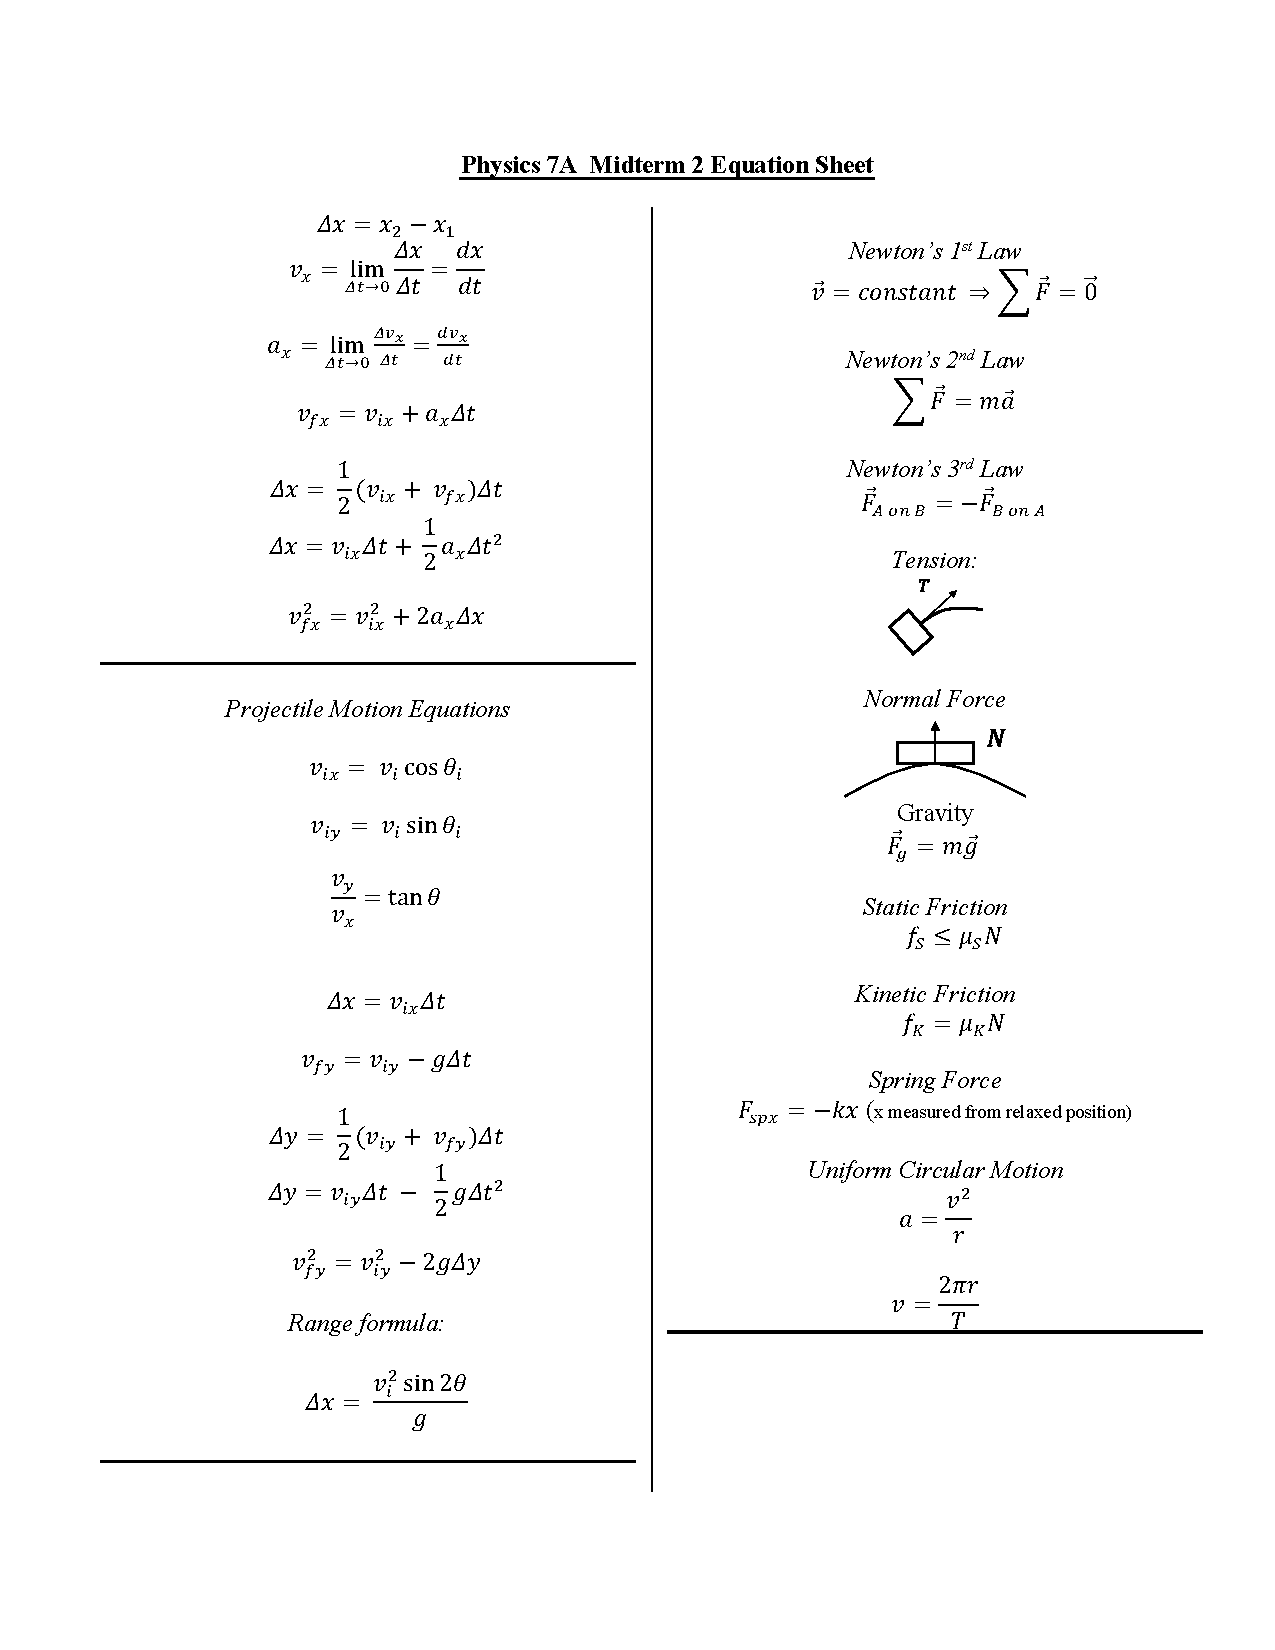
\includepdf[pages=-]{figs/mt2/equation.pdf}

\section{Review Session Problems}

\textbf{1.} \textit{Physics 7A Past Exam Problem}

A block of mass $M$ is resting on an incline that makes an angle $\theta$ with the horizontal, as shown in the diagram. The block is pushed up against a coiled spring that is compressed to a length of $l$. The spring has spring constant $k$ and the natural length of the spring is $L$. The block is initially at rest. 

\fig{figs/mt2/deweese1.png}{Block and Spring on an Incline}{0.65}{0}

For parts a) through d) assume that the incline is frictionless.

a) How much potential energy is stored in the coiled spring?

b) After the spring is released, how far along the incline $D$ does the block move from its initial location before it begins to slide back down again? Express your answer in terms of $M$, $k$, $\theta$, $L$, $l$, and any relevant physical constants.

c) How much work is done by gravity from the time the block is released until the moment the spring reaches its natural length? Express your answer in terms of $M$, $\theta$, $L$, $l$, and any relevant physical constants, and take care with signs.

d) What is the impulse due to the net force on the block from the time the block is released until the moment the spring reaches its natural length? Express your answer in terms of $M$, $k$, $\theta$, $L$, $l$, and any relevant physical constants and indicate whether it points up or down the slope.

e) If the coefficient of kinetic friction between the block and incline were $\mu_k$, then how far up the slope $D'$ would the block get before halting or sliding back down?

\pagebreak

\begin{center}
(Blank Page)
\end{center}

\pagebreak

\textbf{2.} \textit{Physics 7A Past Exam Problem}

Three friends---Alphonse, Beatrice, and Cordelia---are all out ice-skating on a vast, frozen, frictionless pond, where they happen to all be positioned exactly in a single line. Alphonse, with mass $2m$, is initially coasting with constant horizontal velocity $v$ straight for Beatrice, behind whom is Cordelia, while Beatrice and Cordelia, each of mass $m$, are both initially at rest. Neglect air resistance.

\fig{figs/mt2/charman1.png}{Cold Collisions}{0.7}{0}

First, supposing all collisions between friends are impulsive, head-on, and elastic, after colliding, all three friends will eventually be coasting with fixed final velocities:

a) How many collisions occur in all, in what order, and between whom?

b) What is the final velocity of Alphonse? Take velocities directed to the right in
the diagram to be positive.

c) What is the final velocity of Beatrice?

d) What is the final velocity of Cordelia?

\textit{Hint: it may also be simplest to answer the questions out of alphabetical order.}

Suppose instead that friends literally stick together after any collision (perhaps because of their personal attachment, or perhaps just because of the puffy jackets they are wearing):

e) After all collisions, the three friends will all be coasting together at what final velocity?

f) After all collisions, what fraction of their initial total kinetic energy has been lost (ultimately as heat, sound, etc.)?

\pagebreak

\begin{center}
(Blank Page)
\end{center}

\pagebreak

\textbf{3.} \textit{Physics 7A Past Exam Problem}

Consider a wheel of radius $R$ and thickness $d$ that is rolling without slipping down a ramp that forms an angle $\beta$ with respect to the horizontal, as shown in the upper diagram. The wheel has total mass $M$; it consists of an inner disk of uniform density and mass $\frac{1}{2}M$, surrounded by a very thin hollow cylinder of mass $\frac{1}{2}M$. As always, show your work and/or justify your answer for every part of each problem.

\fig{figs/mt2/deweese6.png}{Ramp and Conveyor Belt}{0.5}{0}

a) What is the moment of inertia of the wheel about its axis of symmetry? Express your answer as a function of $M$ and $R$.

b) How much work is done by the normal force on the wheel as it rolls a distance $D$ down the ramp? Express your answer as a function of any combination of $D$, $M$, $R$, $\beta$, and any relevant physical constants.

c) What is the magnitude and direction of the force of friction on the wheel? Express your answer as a function of $M$, $\beta$, and any relevant physical constants.

d) If the wheel starts from rest, what is the angular velocity $\omega$ of the wheel after it has rolled a distance $D$? Express your answer in terms of any combination of $D$, $M$, $R$, $\beta$, and any relevant physical constants.

e) Now consider the same wheel as it rolls without slipping on the conveyor belt shown in the right diagram. If the conveyor belt moves so that the center of mass of the wheel remains in the same place over time, what is the magnitude of the angular acceleration $\alpha$ roller of the large roller at the right of the diagram? The roller turns without slipping on the underside of the belt. Express your answer in terms of $M$, $\beta$, $R$, $r$, and any relevant physical constants.

f) How much work is performed on the wheel by the force of friction after a length $D$ of the conveyor belt has passed under the wheel?

\pagebreak

\begin{center}
(Blank Page)
\end{center}

\pagebreak

\section{Energy}

\textbf{1.} \textit{Physics 7A Past Exam Problem}

\textit{This problem was given in a somewhat longer exam, and may require around 45 minutes to complete.}

Rigelians Kang and Kodos install a gravitational trolley, in which a small spherical capsule slides along an extremely thin, long, massless, frictionless, rigid rod (lying along the $x$ axis). Equidistant from the rod, initially at $x = 0$, $y = \pm L$, are situated the centers of two identical spherical moons that can accelerate the capsule. 

Assume the capsule is a very small, uniform, rigid sphere of radius $a$ and mass $m$, with a hole of negligible size drilled out so that the capsule can slide along the thin rod without friction. The rod is presumed to be fixed in place, by means of other external forces which do not otherwise affect the capsule or the moons. 

Both moons are perfectly spherical, rigid, and uniform in density, each with mass $M$ and an outer radius $R$. The moons are in mutual orbit about each other in the $x = 0$ plane, remaining equidistant from the rod and from each other while revolving in a positive sense about the $+x$ axis, but with negligible gravitational influence from the very small capsule. Both moons also happen to be rotating such that the same points on their respective equators always face each other.

\fig{figs/mt2/charman2.png}{Spacey Transit}{0.55}{0}

a) What is the orbital period $T$ of the moons?

b) What is the total kinetic energy $K$ of the moons?

\textit{Hint: For part (b), remember to consider the kinetic energy from both orbital and spin rotations. }

c) How much work $W$ is done by each moon on the capsule if the capsule is launched with some positive velocity from $x = +8L$, eventually stops at $x = +12L$, then slides all the way to $x = -12L$ before stopping again, then moves (momentarily) to $x = +6L$? 

d) If instead the capsule is released from rest at $x = +4L$, what is the acceleration $a$ of the capsule immediately after being released?

\pagebreak

e) Starting with the same initial conditions as in part (e), what is the velocity $v$ of the capsule when it passes through the origin for the 18th time after its release?

f) Where is the (finite) position $x$ of the equilibrium for the capsule? Is this equilibrium (locally) stable, unstable, or neutral?

g) If the capsule is to be launched from the position $x = +2L$ with some initial velocity, what is the magnitude of the required escape velocity $v_{esc}$ if the capsule is to be able to travel arbitrarily far from the moons?

\pagebreak

\begin{center}
(Blank Page)
\end{center}

\pagebreak

\textbf{2.} \textit{Physics 7A Past Exam Problem}

An alien spaceship hovers in place at a distance $2R$ from the center of the Earth, where $R$ is the Earth’s radius. The alien ship is not in orbit around the Earth, it is holding still and using its rockets to maintain its position.

\fig{figs/mt2/deweese3.png}{Alien Ship}{0.65}{0}

a) The aliens shoot a projectile directly to the right in the diagram and it travels in a perfectly circular orbit around the Earth. What is the speed v of the projectile? Express your answer in terms of some combination of $R$, the mass of the Earth $M$, the mass of the projectile $m$, and any relevant physical constants.

b) What is the period of the orbit described in part a)? If you could not find the speed in part a), you may use the symbol $v$ in your answers for this part and the rest of this problem.

c) If the aliens then shoot a projectile directly away from the Earth at the same speed as you found in part a), how far from the center of the Earth would it rise before it begins to fall back to Earth?

d) If the aliens then shoot a projectile directly to the right as in part a), but at a greater speed $V$ so that it follows a closed orbit that reaches a maximum distance of $4R$ from the center of the Earth, then what is $V$?

e) Given that satellites in geosynchronous orbits (whose orbital period $T$ equals to that of the Earth) travel at a distance of approximately $6R$ from the center of the Earth, then what fraction of a day does it take for the projectile described in parts a) and b) to make one complete orbit? Please simplify into an numerical answer without any variables. 

\pagebreak

\begin{center}
(Blank Page)
\end{center}

\pagebreak

\section{Momentum}

\textbf{1.} \textit{Physics 7A Past Exam Problem}

Supremo the carnival performer is shot from a cannon at an initial speed of $v_0$ and at an angle of $\theta$ from the horizontal, as shown in the diagram. While he is still ascending, he attempts to grab a large bouncy rubber ball placed on a pedestal. Supremo’s mass $M$ is the same as the mass of the ball.

\fig{figs/mt2/deweese4.png}{Supremo, the Human Cannonball}{0.5}{0}

a) If it takes $t = \frac{v_0\sin\theta}{2g}$ after Supremo is shot from the cannon for him to reach the ball, then what are the horizontal and vertical components of Supremo’s velocity immediately before he reaches the ball? Express your answer to this and every later part of this problem in terms of any combination of $M$, $v_0$, $\theta$, and $g$.

b) On his first attempt, the ball bounces off of Supremo’s helmet so that the collision is elastic, and the ball’s velocity immediately after the collision points in the same direction as Supremo’s velocity immediately before the collision. What is the speed of the ball immediately after the impact?

c) Undaunted, Supremo is shot from the cannon a second time. On this second attempt, he gets his hands on the ball, but he can’t hold on and the ball moves horizontally (to the right as viewed in the diagram) immediately after the collision so that the ball has no vertical component to its velocity. Immediately after the collision, if the horizontal component of Supremo’s velocity is exactly one third of the ball’s speed after the collision, then what is the ball’s speed immediately after the collision?

d) In this case, what is the direction and magnitude of the impulse on the ball during the collision?

e) On Supremo’s third attempt, he successfully grabs the ball and holds on to it for the duration of his flight. What is Supremo’s speed immediately after the collision? 

\pagebreak

\begin{center}
(Blank Page)
\end{center}

\pagebreak

\textbf{2.} \textit{Physics 7A Past Exam Problem}

Two boys, each of mass $M$, are standing on a small sled that is itself the same mass $M$. The sled is initially stationary, and it sits on a frictionless frozen pond.

\fig{figs/mt2/deweese5.png}{Two Boys and a Sled}{0.65}{0}

a) One of the boys jumps from one side of the sled while the other boy remains standing on the sled. If the boy jumps so that his horizontal velocity is $v$ with respect to the sled, then what is the final speed of the sled?

b) If the second boy then jumps from the same side of the sled as the first boy, again with a relative horizontal velocity of $v$ with respect to the sled, then what is the final speed of the sled?

c) If the second boy had jumped from the opposite side of the sled after the first boy jumped, then what would the final velocity of the sled be? Clearly indicate which way the sled is moving, if it is moving.

d) Now the boys attach a (massless) scoop to the front of the sled and push the sled so that it is moving with an initial velocity of $V$ with nobody onboard. How fast is the sled moving after it has scooped up a total mass $M$ of snow from the surface of the frozen pond?

e) Now one of the boys removes the scoop and climbs onto the sled with a mass $M$ of snow in a bag. If he throws small snowballs of mass $m_s$ from the back of the sled with horizontal velocity $v_s$ with respect to the sled, then how fast is the sled moving when he runs out of snow? Assume that the sled starts from rest. You may approximate the thrown snowballs as a continuous flow of matter.

\pagebreak

\begin{center}
(Blank Page)
\end{center}

\pagebreak

\textbf{3.} \textit{Physics 7A Past Exam Problem}

Consider three spheres lined up in a row along the x-axis with masses $m_1 = M$, $m_2 = M / 2$, $m_3 = M$. $m_1$ has an initial velocity of $v_0$ in the $+x$ direction, while the other two spheres are initially at rest. $m_1$ has an elastic collision with $m_2$, and then $m_2$ collides and sticks to $m_3$.

\fig{figs/mt2/tbp2.png}{Subsequent Collisions}{0.65}{0}

a) Determine the velocities of $m_1$ and $m_2$ after the first collision. 

b) Determine the velocities of $m_2$ and $m_3$ after the second collision. 

c) After the second collision will $m_1$ collide with the $m_2$, $m_3$ combination? If they do not collide, for what values of $m_3$ would this collision occur? 

\pagebreak

\begin{center}
(Blank Page)
\end{center}

\pagebreak

\section{Rotation}

\textbf{1.} \textit{Physics 7A Past Exam Problem}

On a compact disc (CD), music is coded in a pattern of tiny pits arranged in a track that spirals outward toward the rim of the disc. As the disc spins inside a CD player, the track is scanned at a constant linear speed of v. Because the radius of the track varies as it spirals outward, the angular speed of the disc must change as the CD is played. The equation of a spiral is $r = r_0 + \beta\theta$ where $r_0$ is the initial radius of the spiral at $\theta = 0$, and $\beta$ is a constant. If we take the rotation direction of the CD to be positive, $\beta$ must be positive so that $r$ increases as the disc turns.

\fig{figs/mt2/tbp4.png}{A Spiral on a CD}{0.7}{0}

a) When the disc rotates through a small angle $d\theta$, what is the arc length $ds$ scanned along the track?

b) Integrate $ds$ to find the total distance s scanned along the track as a function of the total angle through which the disc has rotated.

c) Since the track is scanned at a constant linear speed, the distance $s$ is equal to $vt$. Use this to find $\theta$ as a function of time. Two solutions will arise for $\theta$ from a quadratic equation, choose the positive one, and explain why this is the solution to choose.

d) What is the angular velocity $\omega$ as a function of time?

e) What is the angular acceleration $\alpha$ as a function of time? Is it constant?

\pagebreak

\begin{center}
(Blank Page)
\end{center}

\pagebreak

\textbf{2.} \textit{Physics 7A Past Exam Problem}

A cylinder with a mass of $M$, moment of inertia of $I_M$ and radius $R$ rests on a horizontal tabletop. A string is attached to an axle through the center of the cylinder; the cylinder can rotate about the axle as it rolls without slipping. The string runs over a pulley of moment of inertia $I_P$ and radius $r$. A block of $m$ is suspended from the other end of the string, initially at height $h$ above the ground. The system is released from rest. Find the speed of the block just before it hits the ground. 

\textit{Hint: It's easiest to solve this problem with energy. But if you want to solve it with Newton's Laws, be careful with the forces acting on each rotating object.}

\fig{figs/mt2/past.png}{Atwood Machine and Rolling Cylinder}{0.7}{0}

\pagebreak

\begin{center}
(Blank Page)
\end{center}

\pagebreak

\textbf{3.} \textit{Physics 7A Past Exam Problem}

Consider a wheel of radius $r$ and mass $M$ that is rolling along a surface consisting of round segments at the left and right, each with radius $R$, and a flat horizontal section connecting them, as shown in the diagram. The wheel is a solid cylinder of uniform density. The surface on the left and along the flat section at the bottom exert frictional forces on the wheel, but the curved section on the right is frictionless. The wheel starts from rest at the left side of the surface such that its center is at a height $h$ above the flat section. The wheel rolls without slipping all the way to the right side of the flat section. 

Do not assume the wheel is a point mass---it is free to rotate with a moment of inertia $I = \frac{1}{2}Mr^2$. 

\fig{figs/mt2/tbp6.png}{Wheel on a Track}{0.6}{0}

a) What is the speed of the center of mass of the wheel once it reaches the flat section at the bottom? Express your answer as a function of $M$, $h$, $r$, $R$, and any relevant physical constants.

b) How high does the center of mass of the wheel get when it goes up the frictionless slope at the right? Express your answer as a function of any combination of $M$, $h$, $r$, $R$, and any relevant physical constants.

c) What is the power delivered to the wheel from kinetic friction at the instant after the wheel slides from the right onto the horizontal section? Express your answer as a function of the coefficient of kinetic friction $\mu_k$, $r$, $h$, $M$, and any relevant physical constants; and take care with signs.

d) What is the angular acceleration when the wheel is on the horizontal section, after it has slid down from the right? Indicate whether it is clockwise or counterclockwise as viewed in the diagram. Express your answer as a function of $\mu_k$, $r$, and any relevant physical constants.

e) As the wheel then slides along the horizontal section, will the backspin of the wheel cause it to reverse direction? Assume that the width $D$ of the horizontal section is large enough so that the wheel is rolling without slipping by the time it reaches one end or the other. 

\pagebreak

\begin{center}
(Blank Page)
\end{center}

\pagebreak

\end{document}
